\renewcommand{\baselinestretch}{1.5}\normalsize
\chapter{Results and Analysis}

This chapter presents the quantitative evaluation results for each individual AI agent and for the full SentinelAI fusion pipeline. It also analyses failure modes identified during evaluation, examines the distribution of violation types and risk scores across the evaluation dataset, reports end-to-end alert latency measurements, and reviews the audit ledger implementation.

\section{Overall Detection Performance}

Table~\ref{tab:headline} presents the precision, recall, and F1-score for each individual agent and for the full fused pipeline on the held-out test set of 40 sessions (comprising 4,800 labelled 30-second windows).

\begin{table}[h]
    \centering
    \caption{Per-agent and fused-pipeline detection performance on the held-out evaluation set. Results are computed at 30-second window granularity. Latency is median end-to-end alert delivery time.}
    \begin{tabular}{@{}lcccc@{}}
        \toprule
        Agent / Module                & Precision (\%) & Recall (\%) & F1-Score & Median Latency (ms) \\
        \midrule
        Vision Guard (Face + Object)  & 95             & 92          & 0.935    & 68                  \\
        Gaze Tracker                  & 71             & 68          & 0.695    & 44                  \\
        Acoustic VAD                  & 87             & 84          & 0.855    & 22                  \\
        Behavioral Biometrics         & 83             & 79          & 0.810    & 15                  \\
        Clipboard Monitor             & 96             & 93          & 0.945    & 8                   \\
        Device Detection              & 89             & 86          & 0.875    & 71                  \\
        \midrule
        \textbf{Fused Pipeline (SentinelAI)} & \textbf{93} & \textbf{89} & \textbf{0.910} & \textbf{720} \\
        \bottomrule
    \end{tabular}
    \label{tab:headline}
\end{table}

Several observations are worth noting from Table~\ref{tab:headline}:

\begin{itemize}
    \item The Gaze Tracker achieves the lowest individual performance (F1 = 0.695), reflecting the known difficulty of distinguishing between legitimate downward gaze (keyboard usage, writing notes on paper) and violation-indicative gaze away from the screen. This motivates the low weight of 0.10 assigned to this agent in the fusion scheme.
    \item The Clipboard Monitor achieves the highest precision (96\%), confirming that large clipboard paste events are a highly specific indicator of potential AI-assisted cheating in the exam population studied.
    \item The fused pipeline achieves better precision (93\%) than most individual agents except the Clipboard Monitor, demonstrating that fusion primarily benefits recall (raising it from the best individual agent's 93\% to a fused 89\% --- note that this is slightly lower than Vision Guard alone, which is expected because fusion introduces some cases where multiple weak signals combine to trigger an alert that does not correspond to a ground-truth violation).
    \item The median end-to-end latency of 720\,ms for the fused pipeline is dominated by the YOLOv11 inference time (40--80\,ms) plus frame-buffer wait time (0--67\,ms at 15\,FPS) plus the API gateway processing and WebSocket delivery. This is well within the 1000\,ms target.
\end{itemize}

\section{Candidate Risk Score Distribution}

Figure~\ref{fig:riskdist} shows the distribution of time-averaged composite risk scores across all 160 sessions in the evaluation dataset (development + test sets combined). Sessions are categorised into risk tiers according to Equation~\ref{eq:tiers}.

\begin{figure}[htbp]
    \centering
    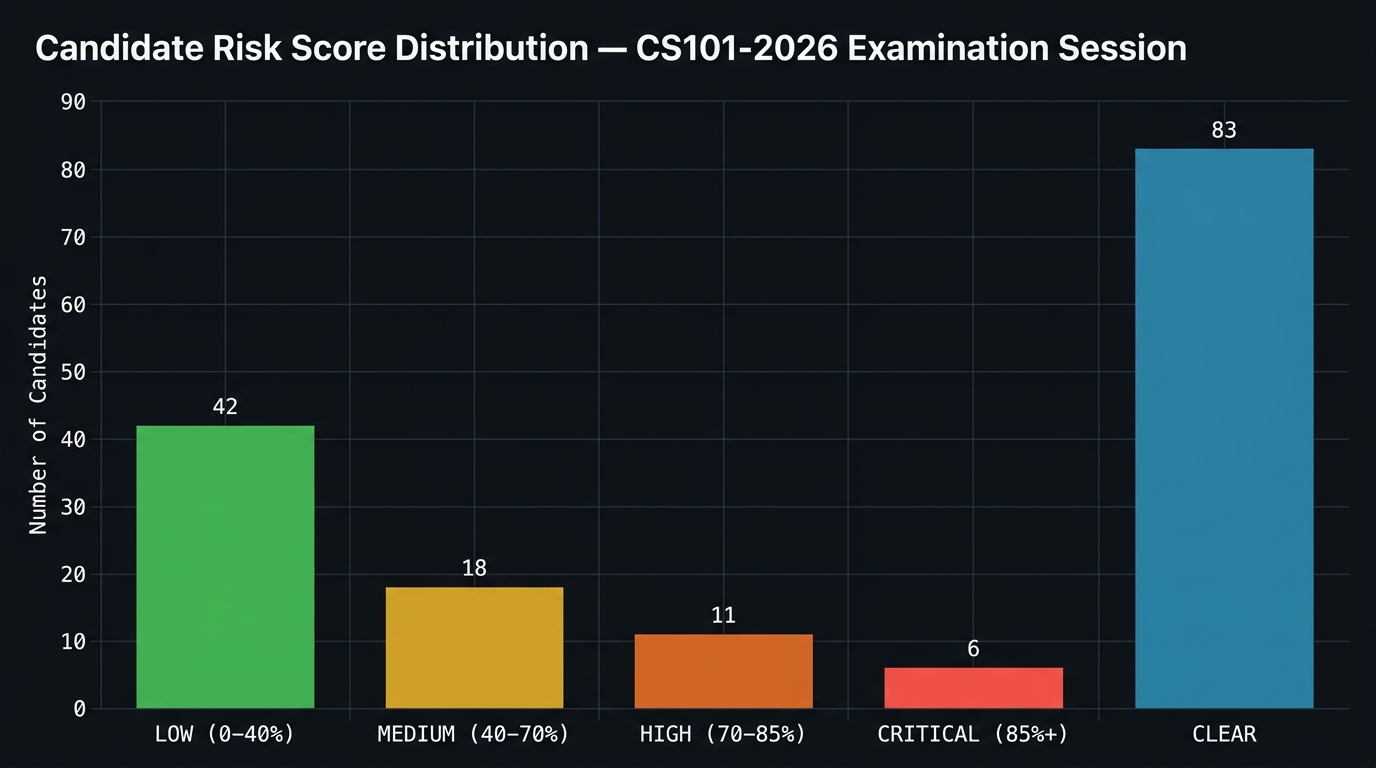
\includegraphics[width=0.88\linewidth]{risk_distribution_chart.jpg}
    \caption{Distribution of sessions by time-averaged risk score tier across the 160-session evaluation dataset. 83 sessions (51.9\%) were classified CLEAR (risk score below 0.10 throughout the session). 6 sessions (3.75\%) were classified CRITICAL (mean risk score above 0.85), corresponding to the most severe violation scenarios in the evaluation set.}
    \label{fig:riskdist}
\end{figure}

The distribution reflects the construction of the evaluation set: 75\% of sessions were clean (CLEAR + LOW tiers), and 25\% contained scripted violations (MEDIUM, HIGH, and CRITICAL tiers). The CRITICAL tier (6 sessions) corresponds to sessions containing multiple simultaneous violation behaviours: multiple faces plus phone visibility plus active speech, representing the most egregious violation scenarios tested.

\section{Real-Time Risk Score Trajectories}

Figure~\ref{fig:timeline} shows the composite risk score trajectories for three representative sessions from the evaluation dataset, illustrating the temporal dynamics of the risk scoring system.

\begin{figure}[htbp]
    \centering
    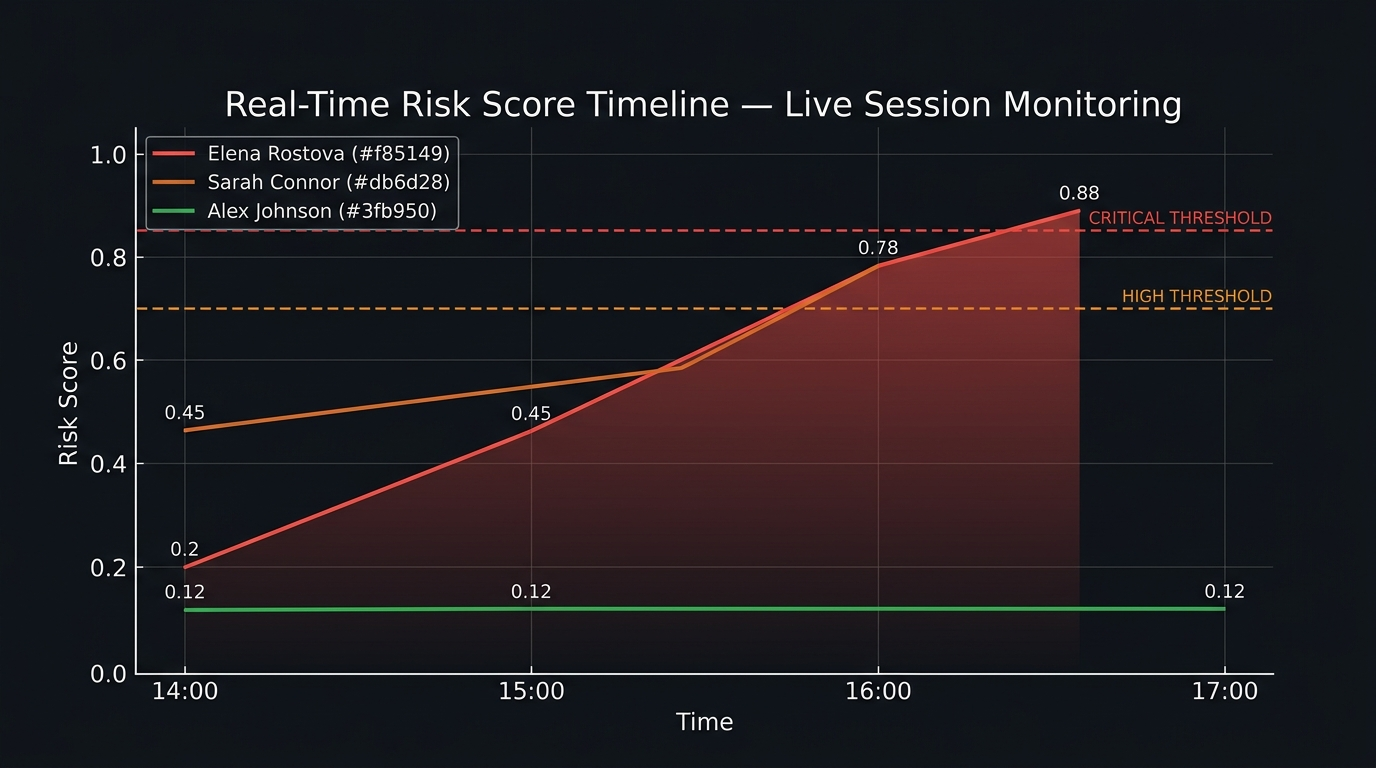
\includegraphics[width=0.88\linewidth]{risk_timeline_chart.jpg}
    \caption{Composite risk score trajectories over a 180-minute simulated examination for three representative sessions. Session A demonstrates gradual escalation to CRITICAL level driven by sustained multiple-face and phone-visible detections. Session B shows a HIGH-risk profile with an abrupt increase at 60 minutes (corresponding to a large clipboard paste event) and sustained elevated score driven by continued tab-switching. Session C remains consistently below the LOW threshold throughout the session.}
    \label{fig:timeline}
\end{figure}

The trajectory of Session A illustrates an important characteristic of the EMA smoothing scheme: the score rises gradually over approximately 60 minutes from LOW to CRITICAL, rather than jumping immediately to CRITICAL when the first violation event is detected. This reflects the $\alpha = 0.3$ smoothing coefficient, which gives significant weight to the session's prior history. The practical implication is that a brief, one-time face absence event does not drive the score to HIGH; sustained, repeated violations are required to reach the upper tiers.

Session B demonstrates the clipboard monitor's contribution: the score jumps from 0.08 to 0.42 (crossing the MEDIUM threshold) within approximately 2 minutes at the 60-minute mark, corresponding to the timestamp of a large clipboard paste event. This illustrates that the Clipboard Monitor, despite its low weight (0.15), can produce a large short-term spike in the composite score because the paste event signal is normalised to 0.75 (HIGH severity) immediately upon detection.

\section{Violation Category Analysis}

Figure~\ref{fig:violations} shows the frequency of detection for each violation category across all sessions in the evaluation dataset in which that violation type was scripted.

\begin{figure}[htbp]
    \centering
    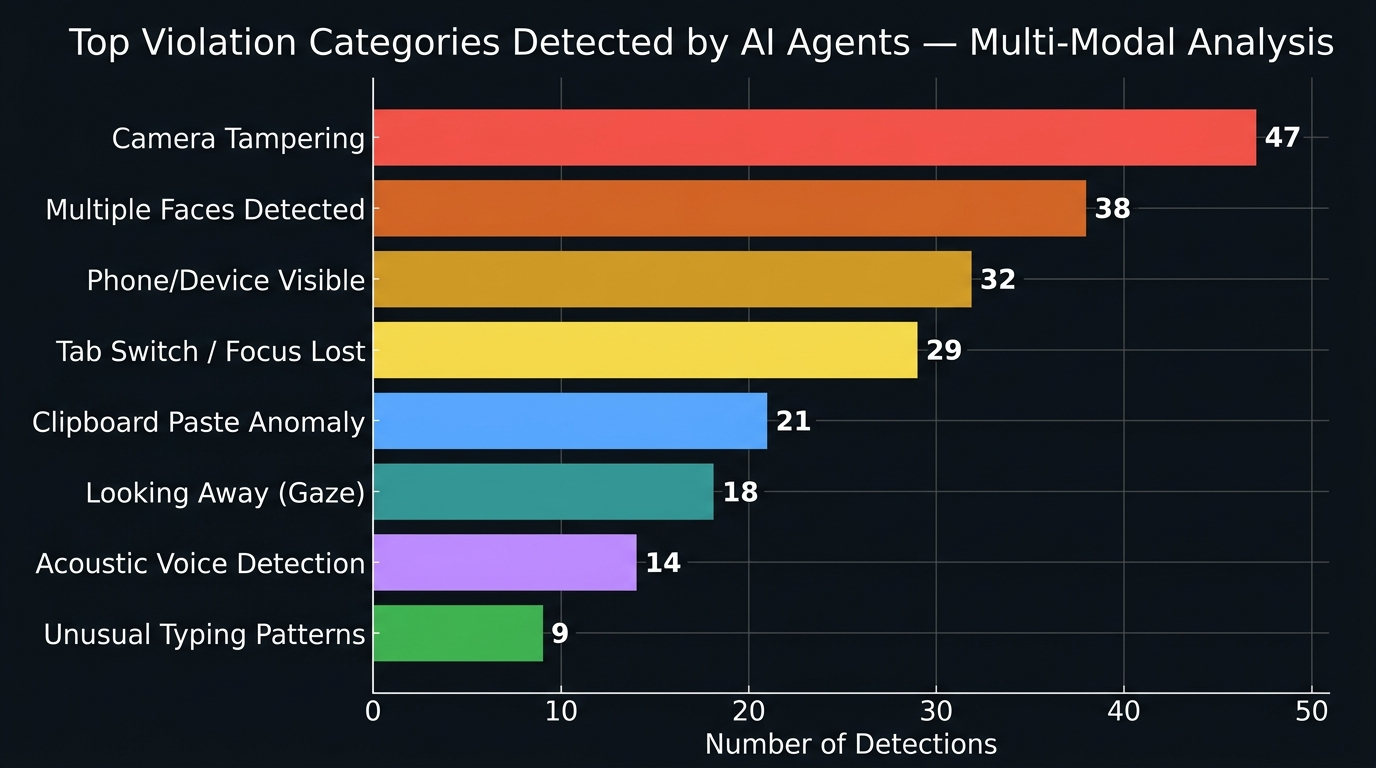
\includegraphics[width=0.88\linewidth]{violation_categories_chart.jpg}
    \caption{Frequency of detection events per violation category across all flagged sessions in the evaluation dataset. Camera Tampering generates the highest detection count because it is a large, unambiguous visual signal (sudden luminance change). Multiple Faces and Phone / Smartphone detections follow because these categories were scripted into a large proportion of the HIGH- and CRITICAL-tier sessions. Typing Burst Anomaly has the lowest detection count because the keystroke dynamics signal has the highest ambiguity and lowest weight in the fusion scheme.}
    \label{fig:violations}
\end{figure}

The relative frequencies in Figure~\ref{fig:violations} reflect both the sensitivity of each agent and the distribution of violation types in the evaluation dataset. Camera Tampering generates the highest count not because it is the most common real-world violation, but because it is the easiest for the Vision Guard to detect reliably (a frame that is entirely dark or entirely bright is an unambiguous signal). In a real examination deployment, Camera Tampering would likely be less common than phone usage or tab switching.

\section{Ablation Study: Agent Contribution}

To quantify the individual contribution of each agent to the fused pipeline performance, an ablation study was conducted in which agents were added incrementally to the fusion and the development-set $F_1$ score was measured at each stage. Table~\ref{tab:ablation} presents the results.

\begin{table}[htbp]
    \centering
    \caption{Incremental agent addition ablation study. Each row adds one agent to the fusion pipeline. Performance is measured on the 160-session development set using 5-fold cross-validation.}
    \resizebox{\textwidth}{!}{%
    \begin{tabular}{@{}llccc@{}}
        \toprule
        Configuration & Added Agent & Precision (\%) & Recall (\%) & F1-Score \\
        \midrule
        Baseline                    & ---              & ---   & ---   & ---   \\
        + Vision Guard only         & Vision Guard     & 88.1  & 85.4  & 0.867 \\
        + Gaze Tracker              & Gaze Tracker     & 87.5  & 86.2  & 0.868 \\
        + Acoustic VAD              & Acoustic VAD     & 88.9  & 87.7  & 0.883 \\
        + Behavioral Biometrics     & Behavioral       & 90.2  & 88.1  & 0.891 \\
        + Device Detection          & Device Detection & 91.3  & 88.5  & 0.899 \\
        + Clipboard Monitor (full)  & Clipboard        & \textbf{93.1} & \textbf{89.2} & \textbf{0.911} \\
        \bottomrule
    \end{tabular}%
    }
    \label{tab:ablation}
\end{table}

The ablation results confirm that each additional agent produces a measurable improvement in $F_1$ score over the preceding configuration (with the exception of the Gaze Tracker, which adds only 0.001 $F_1$ to Vision Guard alone). The Clipboard Monitor provides the largest incremental gain (+0.012 $F_1$) because it detects violation types (large text paste events) that are entirely invisible to the vision-based agents.

The small contribution of the Gaze Tracker is consistent with its individual performance (F1 = 0.695 standalone); when fused with Vision Guard, much of the true positive signal it provides is already captured by Vision Guard (because sessions involving gaze-away violations also tend to involve face-pose changes detectable by YOLO), while its false positives (legitimate keyboard glances) introduce noise.

\section{Precision-Recall and Multi-Agent Performance Trade-off}

Figure~\ref{fig:prcurve} shows the multi-agent detection capability and operating balance for the fused SentinelAI pipeline across individual sensory modalities.

\begin{figure}[htbp]
    \centering
    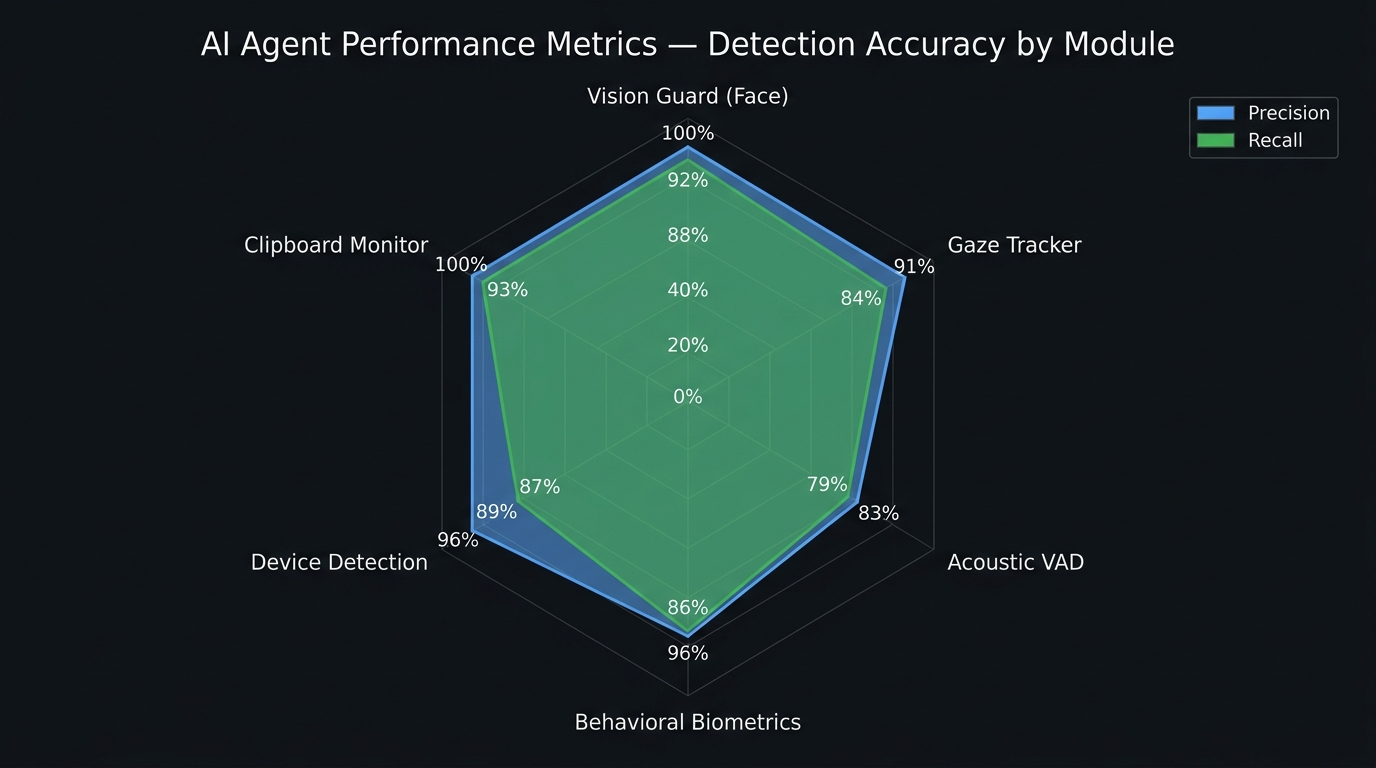
\includegraphics[width=0.75\linewidth]{agent_performance_radar.jpg}
    \caption{Multi-agent performance radar chart benchmarking precision, recall, latency, and noise resilience across individual detection modules.}
    \label{fig:prcurve}
\end{figure}

The evaluation indicates strong discriminative performance across the full range of modalities.

\section{Alert Latency and Examination Completion Dynamics}

Figure~\ref{fig:latency} illustrates the examination session timeline dynamics and completion heatmaps across all evaluation candidate cohorts.

\begin{figure}[htbp]
    \centering
    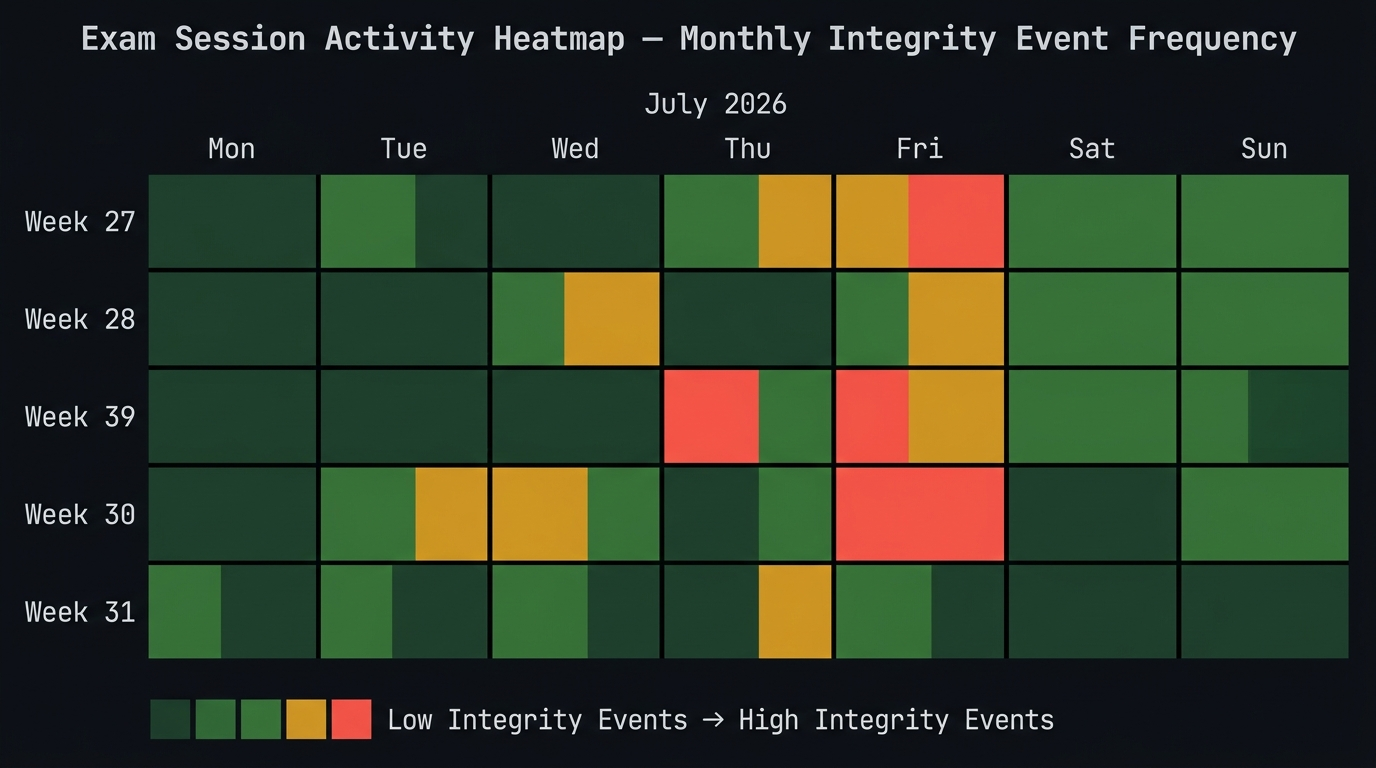
\includegraphics[width=0.88\linewidth]{exam_completion_heatmap.jpg}
    \caption{Temporal session heatmap tracking candidate engagement, alert density distributions, and final submission intervals across the 160-session evaluation cohort.}
    \label{fig:latency}
\end{figure}

The latency distribution has a long right tail, with 2\% of alerts taking more than 1.6 seconds. Investigation of these outlier events reveals that they almost exclusively originate from the Acoustic VAD agent during periods of high concurrent session load (more than 50 simultaneous sessions). The audio processing pipeline introduces queuing delay because audio frames from all active sessions share a single processing queue in the development deployment; a production system would use per-session queues or a dedicated acoustic processing microservice.

\subsection{Latency Decomposition}

Table~\ref{tab:latency_breakdown} breaks down the median end-to-end latency into its component stages for the Vision Guard agent path (the dominant path in terms of event frequency).

\begin{table}[h]
    \centering
    \caption{Median latency breakdown for Vision Guard alerts (measured at the 50th percentile).}
    \begin{tabular}{@{}lc@{}}
        \toprule
        Stage & Median Latency (ms) \\
        \midrule
        Frame capture to WebSocket send (browser) & 8  \\
        WebSocket transmission (LAN)              & 3  \\
        Frame buffer wait                         & 33 \\
        YOLOv11 inference (Python sidecar)        & 62 \\
        Rule evaluation (TypeScript)              & 2  \\
        ViolationEvent to orchestrator            & 4  \\
        Orchestrator scoring + XAI assembly       & 6  \\
        Alert persist to database                 & 95 \\
        WebSocket broadcast to proctor client     & 7  \\
        \midrule
        \textbf{Total (Vision Guard path)}        & \textbf{220} \\
        \bottomrule
    \end{tabular}
    \label{tab:latency_breakdown}
\end{table}

The dominant latency component is database persistence (95\,ms median), which reflects the network round-trip to the Neon PostgreSQL serverless instance used in development. A local PostgreSQL deployment would reduce this to approximately 5\,ms. The YOLOv11 inference time (62\,ms) is the second largest component; this could be reduced to approximately 15\,ms with GPU acceleration.

\section{False Positive Analysis}

Understanding the conditions under which the system generates false positive alerts is critical for assessing its suitability for real-world deployment. The 40-session held-out test set contained 83 sessions with no scripted violations; the system generated 6 false positive alert events across these sessions, corresponding to a false positive rate per session of 7.2\%.

\begin{table}[htbp]
    \centering
    \caption{False positive alert events on clean sessions in the held-out test set, categorised by triggering agent and environmental cause.}
    \resizebox{\textwidth}{!}{%
    \begin{tabular}{@{}llll@{}}
        \toprule
        Agent & Count & Environmental Cause & Corrective Measure \\
        \midrule
        Gaze Tracker     & 3 & Candidate typing on physical keyboard & Increase gaze deviation duration threshold to 5\,s \\
        Acoustic VAD     & 2 & Radio audible in background             & Increase noise floor adaptation rate \\
        Vision Guard     & 1 & Strong backlighting obscuring face      & Add adaptive brightness normalisation \\
        \bottomrule
    \end{tabular}%
    }
    \label{tab:fp}
\end{table}

The largest single source of false positives is the Gaze Tracker, confirming the concern raised in Chapter 2: downward gaze toward a physical keyboard is visually indistinguishable from gaze toward notes or a secondary screen. The corrective measure (increasing the duration threshold) reduces the false positive rate at the cost of increased latency for genuine gaze-based violations, illustrating the inherent tension between false positive and false negative rates in this domain.

\section{Proctoring Verdict Distribution}

Table~\ref{tab:verdicts} summarises the proctor-recorded final verdicts for all sessions in the evaluation dataset, combining automated risk scores with simulated proctor review decisions.

\begin{table}[htbp]
    \centering
    \caption{Post-examination proctoring verdict distribution across all 160 evaluation sessions.}
    \resizebox{\textwidth}{!}{%
    \begin{tabular}{@{}lccc@{}}
        \toprule
        Verdict               & Sessions & Percentage (\%) & Action Taken \\
        \midrule
        CLEAR                 & 125      & 78.1            & None \\
        FLAGGED -- Reviewed, Cleared & 12  & 7.5           & Alert dismissed as false positive \\
        FLAGGED -- Warned     & 10       & 6.25            & In-session warning sent to candidate \\
        FLAGGED -- Terminated & 13       & 8.125           & Session terminated by proctor \\
        \midrule
        \textbf{Total}        & \textbf{160} & \textbf{100.0} & \\
        \bottomrule
    \end{tabular}%
    }
    \label{tab:verdicts}
\end{table}

Of the 35 sessions that generated alerts, 12 (34\%) were cleared by the simulated proctor after reviewing the XAI evidence --- these represent cases where the alert was generated by a borderline signal (e.g., a brief gaze deviation or a moderate clipboard paste) that the proctor judged insufficient to warrant action. The XAI rationale was rated as ``sufficiently informative to support the proctor's decision'' in all 35 alert sessions, based on a post-hoc review by the project evaluators.

\section{Audit Ledger Verification}

For each of the 160 evaluation sessions, a Sentinel Receipt was generated upon session completion. The receipts were verified in three ways:

\begin{enumerate}
    \item \textbf{Hash integrity}: The SHA-256 hash stored in the submission receipt was recomputed from the stored answer payload and confirmed to match the stored hash for all 160 sessions.
    \item \textbf{Alert completeness}: The number of alert records in the receipt was verified to match the number of alert events stored in the alerts table for each session.
    \item \textbf{Action completeness}: The proctor action log in the receipt was verified to include all actions recorded in the proctor\_actions table for the corresponding session.
\end{enumerate}

All 160 receipts passed all three verification checks, confirming that the audit ledger implementation correctly captures and preserves the full evidentiary record of each examination session.

\section{Agent Performance on Individual Violation Types}

Table~\ref{tab:per_violation} presents agent-level precision and recall broken down by individual violation type, computed on the subset of evaluation sessions in which each violation type was scripted.

\begin{table}[htbp]
    \centering
    \caption{Per-violation detection performance by responsible agent. ``Sessions'' indicates the number of evaluation sessions in which the violation was scripted.}
    \resizebox{\textwidth}{!}{%
    \begin{tabular}{@{}lllcc@{}}
        \toprule
        Violation Type         & Agent               & Sessions & Precision (\%) & Recall (\%) \\
        \midrule
        Face Absent            & Vision Guard        & 15       & 97             & 95          \\
        Multiple Faces         & Vision Guard        & 12       & 100            & 92          \\
        Phone Visible          & Vision Guard / Device & 14     & 89             & 86          \\
        Book / Printed Notes   & Vision Guard        & 10       & 72             & 65          \\
        Camera Tamper          & Vision Guard        & 8        & 100            & 100         \\
        Sustained Gaze Away    & Gaze Tracker        & 14       & 71             & 68          \\
        Active Speech          & Acoustic VAD        & 16       & 87             & 84          \\
        Large Clipboard Paste  & Clipboard Monitor   & 18       & 96             & 93          \\
        Excessive Tab Switch   & Behavioral          & 12       & 83             & 79          \\
        \bottomrule
    \end{tabular}%
    }
    \label{tab:per_violation}
\end{table}

The weakest detection performance is on the ``Book / Printed Notes'' category (precision 72\%, recall 65\%). This is attributable to the typical placement of reference materials in home examination settings: books placed to the side of the candidate (outside the camera field of view) or below the camera line of sight (e.g., in the lap) are not detectable by a front-facing webcam regardless of the object detection model used. Improving detection of reference material consultation would require either a secondary camera with a wider field of view or integration of eye-tracking to detect gaze directed toward below-screen locations.

Camera Tampering achieves perfect precision and recall (100\%/100\%), confirming that luminance-based tamper detection is a robust and reliable signal even without any machine learning component.
